\documentclass[conference,letterpaper]{IEEEtran}

\usepackage[T1]{fontenc}
\usepackage[utf8]{inputenc}
\usepackage{mathptmx}
\usepackage[spanish,es-noshorthands,es-tabla,es-nodecimaldot]{babel}
\usepackage{cite}
\usepackage{amsmath,amssymb}
\usepackage{graphicx}
\usepackage{booktabs}
\usepackage{array}
\usepackage{tabularx}
\usepackage[table]{xcolor}
\usepackage{tikz}
\usetikzlibrary{arrows.meta,positioning,fit,calc}
\usepackage{pgfplots}
\pgfplotsset{compat=1.18}
\usepackage{microtype}
\usepackage{xurl}
\usepackage[hidelinks]{hyperref}

\graphicspath{{../tesina/images/}}

\addto\captionsspanish{%
  \renewcommand{\figurename}{Fig.}%
  \renewcommand{\tablename}{Tabla}%
  \renewcommand{\IEEEkeywordsname}{Palabras clave}%
}

\definecolor{okblue}{RGB}{0,114,178}
\definecolor{okverm}{RGB}{213,94,0}
\definecolor{okgreen}{RGB}{0,158,115}
\definecolor{okgray}{RGB}{110,110,110}
\definecolor{heat}{RGB}{213,94,0}

\newcommand{\Fone}{$F_1$}
\newcommand{\hm}[2]{\cellcolor{heat!\the\numexpr #1*70/4741+6\relax}#2}
\newcommand{\hz}{\textcolor{okgray}{--}}

\begin{document}

\title{DoctorMaíz: diagnóstico fitosanitario sin conexión de la hoja de maíz en el teléfono y evaluación de su generalización entre fuentes de datos}

\author{%
\IEEEauthorblockN{Josías Abner Rivas Fuentes, David Alejandro Deras Cerros y Elmer Edenilson Rosales Molina}
\IEEEauthorblockA{Escuela de Ingeniería de Sistemas Informáticos, Facultad de Ingeniería y Arquitectura\\
Universidad de El Salvador, San Salvador, El Salvador}
}

\maketitle

\begin{abstract}
Los pequeños productores de maíz de El Salvador diagnostican a simple vista las enfermedades, plagas y deficiencias de la hoja, con poca asistencia técnica y sin conexión estable en la parcela. Este artículo presenta DoctorMaíz, una aplicación Android que clasifica nueve condiciones de la hoja de maíz con una red convolucional cuantizada a enteros de 8 bits que se ejecuta en el propio teléfono. Se consolidó un corpus de 33\,429 imágenes de 11 repositorios públicos, auditado con huellas SHA-256 de archivo y de píxeles y con registro de procedencia. El modelo seleccionado, EfficientNet-Lite0, alcanzó un Macro \Fone{} de 0.9480 y una exactitud de 97.81\% en 5\,015 imágenes de prueba. Su versión Int8 de 3.74\,MB conservó ese desempeño (0.9489) con medianas de 98\,ms de preprocesado y 23\,ms de inferencia en un teléfono de gama media. Un detector fuera de distribución basado en la distancia de Mahalanobis relativa y una regla de abstención por confianza evitan emitir diagnósticos sobre imágenes ajenas al dominio. La evaluación de la generalización expone el límite principal del sistema. Con validación cruzada agrupada por fuente el Macro \Fone{} cae de 0.9311 a 0.6026, en 97 fotografías de campo externas el modelo acierta 41, y al ocultar el centro de la imagen conserva 79.46\% de exactitud. Parte de lo aprendido corresponde a la procedencia de las imágenes y no a los síntomas, lo que orienta el trabajo futuro hacia la recolección de fotografías locales mediante el módulo de aportes voluntarios que incluye la aplicación.
\end{abstract}

\begin{IEEEkeywords}
Aprendizaje por atajos, cuantización, detección fuera de distribución, EfficientNet, enfermedades foliares del maíz, inferencia en el dispositivo, redes neuronales convolucionales, validación agrupada por fuente.
\end{IEEEkeywords}

\section{Introducción}

\IEEEPARstart{E}{l} maíz (\textit{Zea mays} L.) es la base de la alimentación de las familias campesinas de El Salvador. La agricultura aporta el 5.6\% del producto interno bruto del país \cite{bcr2023}, y el 82.1\% de los productores trabaja parcelas menores de 1.4\,ha bajo un régimen de subsistencia que depende de las lluvias \cite{mag2023}. Las pérdidas mejor documentadas son climáticas. En el ciclo 2023--2024 se perdieron unos 1.46 millones de quintales, el 9.8\% de la producción \cite{edh2024}, y en el ciclo 2024--2025 la cosecha cubrió 10.9 de los 18.8 millones de quintales requeridos \cite{elmundo2025}. El efecto de las enfermedades foliares, las plagas y las deficiencias nutricionales no está cuantificado a escala nacional, y la evidencia disponible es puntual. En ensayos del CENTA, los sitios con presión de mancha de asfalto rindieron cerca de 51\% menos que los sitios sin la enfermedad \cite{deras2014}, y en un ensayo en La Libertad el control intensivo de plagas y enfermedades elevó el rendimiento 15\% pero redujo la utilidad neta \cite{eash2019}.

En la parcela, el diagnóstico se hace a simple vista y varias condiciones se confunden entre sí. Una hoja amarillenta puede deberse a falta de nitrógeno o a una virosis, y las lesiones del tizón foliar se parecen a las de la mancha gris. La asistencia técnica pública no alcanza a cubrir a los productores dispersos, y sin un diagnóstico la recomendación del agroservicio tiende a ser un agroquímico de amplio espectro, aun cuando el síntoma se debe a una deficiencia del suelo \cite{centa2022}.

Las aplicaciones de diagnóstico por visión artificial atienden solo en parte esta necesidad. La mayoría procesa la fotografía en un servidor, lo que exige una cobertura celular que falta en muchas zonas rurales. Los modelos convencionales requieren más memoria y cómputo de los que ofrecen los teléfonos de gama baja y media. Además, los clasificadores entrenados con imágenes de laboratorio pierden gran parte de su exactitud en fotografías de campo \cite{mohanty2016,ferentinos2018,ahmad2023}, y una partición aleatoria de un mismo repositorio no revela esa pérdida porque el modelo puede apoyarse en el fondo o en la cámara en lugar de la lesión \cite{geirhos2020,noyan2022}.

Este trabajo aborda la siguiente pregunta. ¿En qué medida puede una aplicación móvil que funciona sin conexión, en teléfonos de gama baja o media, identificar problemas fitosanitarios en fotografías de hojas de maíz, abstenerse cuando la imagen no es confiable y orientar al productor sobre el manejo del cultivo? Las contribuciones son cuatro.
\begin{enumerate}
\item Un corpus consolidado y público de 33\,429 imágenes de nueve condiciones de la hoja de maíz, procedente de 11 repositorios, con auditoría de duplicados por doble huella SHA-256 y registro de procedencia por imagen.
\item Un protocolo de evaluación que contrasta la partición estratificada con la validación agrupada por fuente, la retención de fuentes completas, un conjunto de fotografías de campo externas, una métrica de disparidad entre entornos y una ablación espacial, y que cuantifica cuánto del desempeño se debe a la procedencia.
\item Un sistema móvil sin conexión con un modelo Int8 de 3.74\,MB, un detector fuera de distribución basado en la distancia de Mahalanobis relativa y una regla de abstención, cuya paridad con el modelo evaluado se verificó en el dispositivo.
\item Un módulo de aportes voluntarios con sincronización diferida, que sienta la base de un conjunto de datos nacional.
\end{enumerate}

La Sección~\ref{sec:relacionados} revisa los trabajos relacionados. La Sección~\ref{sec:metodos} describe el corpus, el entrenamiento, el protocolo de evaluación y el despliegue. La Sección~\ref{sec:resultados} presenta los resultados, la Sección~\ref{sec:discusion} los discute y la Sección~\ref{sec:conclusiones} concluye.

\section{Trabajos relacionados}\label{sec:relacionados}

\subsection{Clasificación de enfermedades foliares}
El repositorio PlantVillage \cite{hughes2015} impulsó una serie de clasificadores convolucionales con exactitudes superiores al 99\% en partición aleatoria. Mohanty \textit{et~al.} \cite{mohanty2016} reportaron 99.35\% sobre ese repositorio y una caída a 31.4\% en imágenes de otra procedencia. Ferentinos \cite{ferentinos2018} observó una degradación similar al entrenar con imágenes de laboratorio y evaluar con imágenes de campo, y Barbedo \cite{barbedo2018} mostró que la variedad del conjunto de datos pesa tanto como su tamaño. Para el maíz, DeChant \textit{et~al.} \cite{dechant2017} detectaron el tizón foliar en imágenes de campo, y PlantDoc \cite{singh2020} reunió fotografías de campo de varios cultivos precisamente por las limitaciones de las imágenes de laboratorio. Ahmad \textit{et~al.} \cite{ahmad2023} estudiaron de forma sistemática la generalización entre condiciones controladas y de campo y concluyeron que las particiones aleatorias sobrestiman el desempeño real.

\subsection{Aprendizaje por atajos y sesgo de procedencia}
Un modelo puede acertar apoyándose en señales correlacionadas con la etiqueta que no forman parte del fenómeno, como el fondo, la iluminación o una marca de agua \cite{geirhos2020}. Lapuschkin \textit{et~al.} \cite{lapuschkin2019} documentaron estos predictores de tipo \textit{Clever Hans} con métodos de atribución, y Noyan \cite{noyan2022} mostró que en PlantVillage un clasificador entrenado solo con píxeles del fondo supera ampliamente al azar. Cuando la procedencia y la clase están asociadas, como ocurre al combinar repositorios que aportan una o dos clases cada uno, la validación agrupada por fuente es la forma directa de medir este efecto.

\subsection{Modelos ligeros y cuantización}
Las arquitecturas diseñadas para dispositivos móviles reducen el cómputo mediante convoluciones separables en profundidad \cite{howard2017,sandler2018}, escalado compuesto \cite{tan2019} y operaciones con menor costo de acceso a memoria \cite{ma2018}. La cuantización a enteros de 8 bits reduce el tamaño del modelo a cerca de una cuarta parte y acelera la inferencia en CPU \cite{jacob2018}, y la cuantización por canal de salida limita la pérdida de exactitud en las convoluciones separables \cite{krishnamoorthi2018}.

\subsection{Detección fuera de distribución y abstención}
Un clasificador con salida \textit{softmax} siempre elige una de sus clases, incluso ante imágenes sin relación con el dominio. La probabilidad máxima es una línea base sencilla para detectar estas entradas \cite{hendrycks2017}. Lee \textit{et~al.} \cite{lee2018} propusieron la distancia de Mahalanobis sobre las representaciones internas, Ren \textit{et~al.} \cite{ren2021} la corrigieron restando la distancia a una gaussiana de fondo y Müller y Hein \cite{mueller2025} mostraron que normalizar las representaciones mejora la detección. Los ensambles también mejoran la calibración de la incertidumbre \cite{lakshminarayanan2017}.

Pocos trabajos combinan el despliegue sin conexión en teléfonos de gama media con una evaluación por fuente y un mecanismo de abstención. Este trabajo integra los tres elementos y reporta el desempeño fuera de la partición de entrenamiento junto al desempeño en ella.

\section{Materiales y métodos}\label{sec:metodos}

\subsection{Corpus y taxonomía}
El sistema distingue nueve clases mutuamente excluyentes, que son tres enfermedades fúngicas (roya común, \textit{Puccinia sorghi}, tizón foliar del norte, \textit{Exserohilum turcicum}, y mancha gris, \textit{Cercospora zeae-maydis}), la necrosis letal del maíz, causada por la coinfección del MCMV con un potyvirus \cite{mahuku2015}, el gusano cogollero (\textit{Spodoptera frugiperda}), las deficiencias de nitrógeno, fósforo y potasio, y la hoja sana. La Fig.~\ref{fig:clases} muestra un ejemplo de cada clase.

\begin{figure}[!t]
\centering
\setlength{\tabcolsep}{1pt}
\begin{tabular}{ccc}
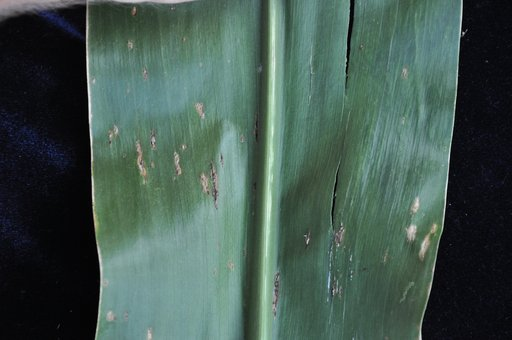
\includegraphics[width=0.315\columnwidth,height=0.22\columnwidth]{dataset-classes/common_rust.jpg} &
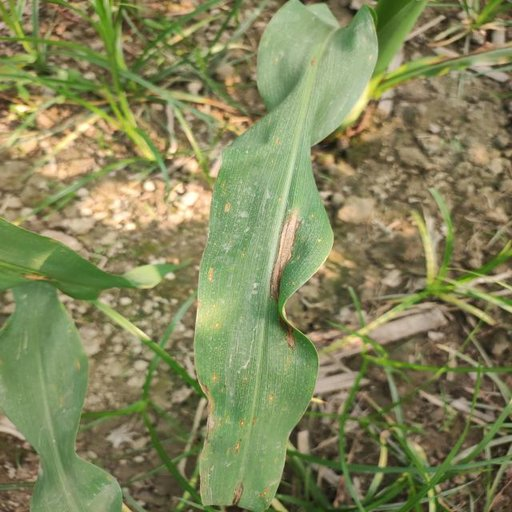
\includegraphics[width=0.315\columnwidth,height=0.22\columnwidth]{dataset-classes/northern_corn_leaf_blight.jpg} &
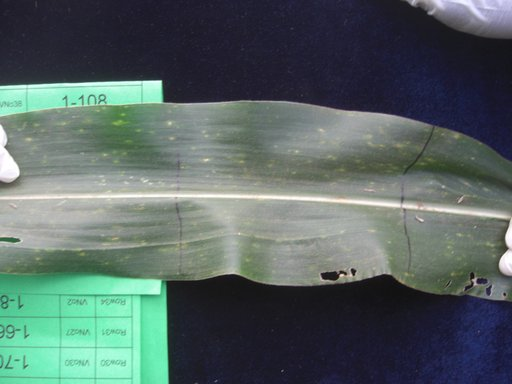
\includegraphics[width=0.315\columnwidth,height=0.22\columnwidth]{dataset-classes/gray_leaf_spot.jpg} \\[-1pt]
\scriptsize (a) Roya común & \scriptsize (b) Tizón foliar & \scriptsize (c) Mancha gris \\
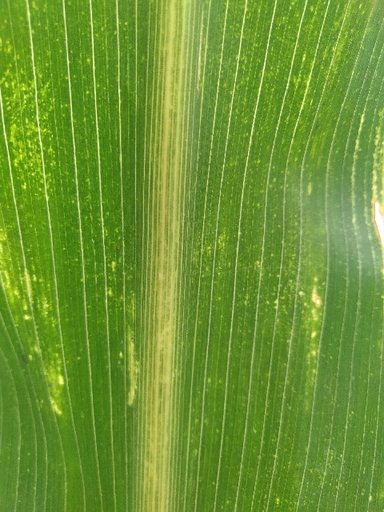
\includegraphics[width=0.315\columnwidth,height=0.22\columnwidth]{dataset-classes/lethal_necrosis.jpg} &
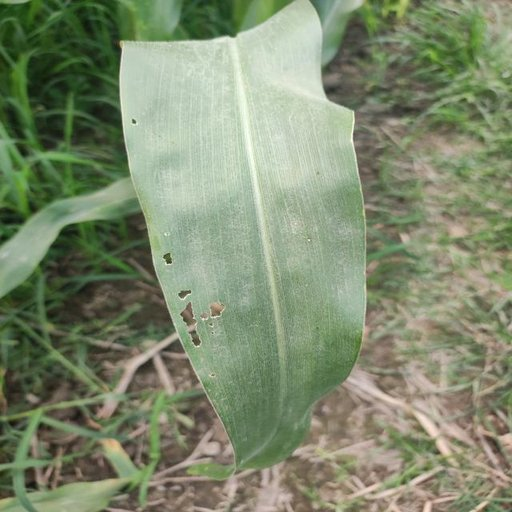
\includegraphics[width=0.315\columnwidth,height=0.22\columnwidth]{dataset-classes/fall_armyworm.jpg} &
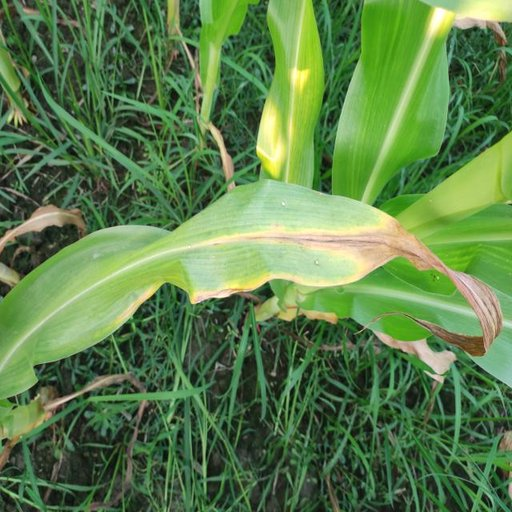
\includegraphics[width=0.315\columnwidth,height=0.22\columnwidth]{dataset-classes/nitrogen_deficiency.jpg} \\[-1pt]
\scriptsize (d) Necrosis letal & \scriptsize (e) Gusano cogollero & \scriptsize (f) Deficiencia de N \\
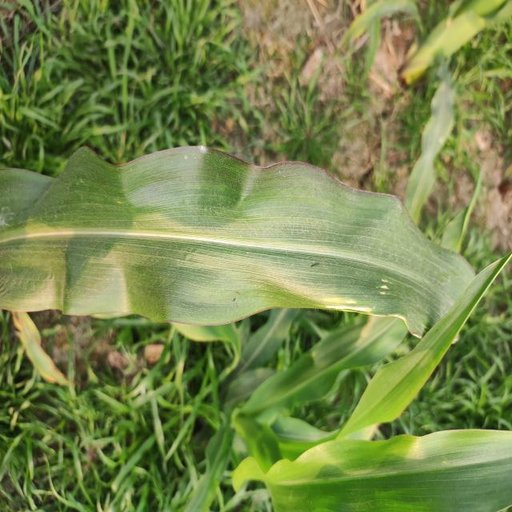
\includegraphics[width=0.315\columnwidth,height=0.22\columnwidth]{dataset-classes/phosphorus_deficiency.jpg} &
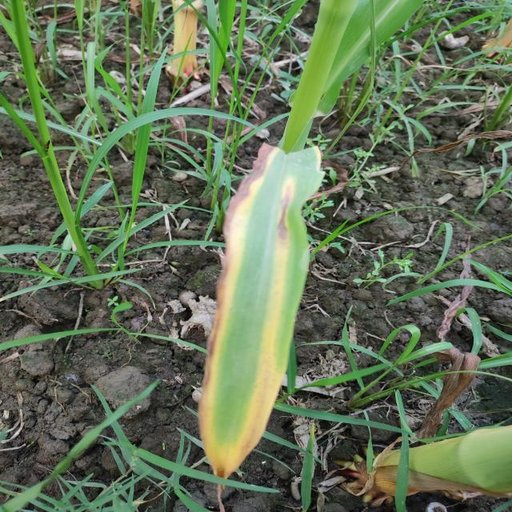
\includegraphics[width=0.315\columnwidth,height=0.22\columnwidth]{dataset-classes/potassium_deficiency.jpg} &
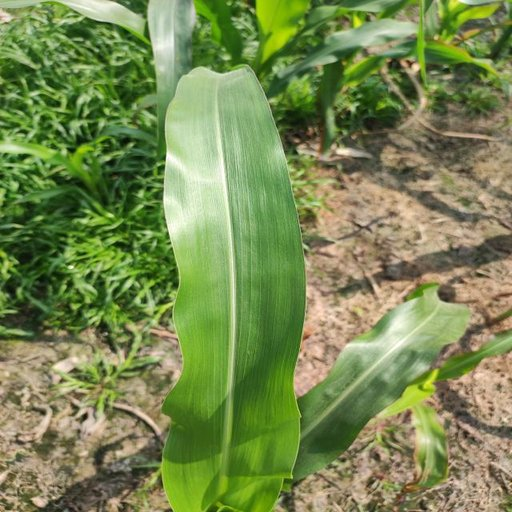
\includegraphics[width=0.315\columnwidth,height=0.22\columnwidth]{dataset-classes/healthy.jpg} \\[-1pt]
\scriptsize (g) Deficiencia de P & \scriptsize (h) Deficiencia de K & \scriptsize (i) Hoja sana
\end{tabular}
\caption{Ejemplos de las nueve clases del corpus.}
\label{fig:clases}
\end{figure}

El corpus reúne 33\,429 imágenes de 11 repositorios públicos (Tabla~\ref{tab:fuentes}) y conserva la licencia declarada por cada uno. Está desbalanceado, con 8\,740 imágenes de hoja sana frente a 621 de deficiencia de potasio (relación 14.1:1), y sus resoluciones van de unos 256\,px en las imágenes de laboratorio a 3\,000--5\,000\,px en varias fuentes de campo. Solo tres clases tienen imágenes tomadas en laboratorio sobre fondo controlado, que suman 3\,551 (10.6\% del corpus). La procedencia y la clase están asociadas (Tabla~\ref{tab:fuente_clase}). Varias fuentes aportan una sola clase, la roya común procede en un 95.3\% del laboratorio y una sola fuente (S1) aporta el 36.3\% de las imágenes.

\begin{table}[!t]
\caption{Fuentes del corpus}
\label{tab:fuentes}
\centering
\scriptsize
\setlength{\tabcolsep}{3pt}
\begin{tabularx}{\columnwidth}{@{}l>{\raggedright\arraybackslash}Xlrl@{}}
\toprule
& \textbf{Identificador} & \textbf{Licencia} & \textbf{Imág.} & \textbf{Entorno} \\
\midrule
S1 & \path{maize-beans-tomatoes-africa} & Apache 2.0, CC & 12\,136 & Campo \\
S2 & \path{maize-diseases} & CC BY-NC-SA 4.0 & 6\,989 & Mixto \\
S3 & \path{multicrop-disease-maiz} & CC BY 4.0 & 5\,816 & Mixto \\
S4 & \path{corn-leaf-roboflow} & CC BY 4.0 & 2\,919 & Campo \\
S5 & \path{cropdg-unified-multidomain} & CC BY-NC-SA 4.0 & 2\,562 & Mixto \\
S6 & \path{maize-in-field-dataset} & CC BY-NC-SA 4.0 & 852 & Campo \\
S7 & \path{maize-2-roboflow} & CC BY 4.0 & 846 & Campo \\
S8 & \path{corn-leaf-diseases-classification-roboflow} & CC BY 4.0 & 480 & Mixto \\
S9 & \path{maize-nutrient-deficiency} & CC BY 4.0 & 340 & Campo \\
S10 & \path{maize-leaf-roboflow} & CC BY 4.0 & 331 & Campo \\
S11 & \path{maize-deficiency-scanner-roboflow} & CC BY 4.0 & 158 & Campo \\
\midrule
& \textbf{Total} & & \textbf{33\,429} & \\
\bottomrule
\end{tabularx}
\end{table}

\begin{table*}[!t]
\caption{Imágenes por clase y fuente. La intensidad del color es proporcional al número de imágenes}
\label{tab:fuente_clase}
\centering
\footnotesize
\setlength{\tabcolsep}{4.2pt}
\begin{tabular}{@{}l*{11}{r}rr@{}}
\toprule
\textbf{Clase} & \textbf{S1} & \textbf{S2} & \textbf{S3} & \textbf{S4} & \textbf{S5} & \textbf{S6} & \textbf{S7} & \textbf{S8} & \textbf{S9} & \textbf{S10} & \textbf{S11} & \textbf{Total} & \textbf{Lab.} \\
\midrule
Hoja sana & \hm{2310}{2\,310} & \hm{4741}{4\,741} & \hz & \hm{456}{456} & \hm{1161}{1\,161} & \hz & \hz & \hz & \hm{72}{72} & \hz & \hz & 8\,740 & 0\% \\
Tizón foliar & \hm{4223}{4\,223} & \hm{1056}{1\,056} & \hz & \hm{523}{523} & \hm{888}{888} & \hm{140}{140} & \hz & \hz & \hz & \hz & \hz & 6\,830 & 13.0\% \\
Necrosis letal & \hm{3184}{3\,184} & \hz & \hm{3231}{3\,231} & \hz & \hz & \hz & \hz & \hz & \hz & \hz & \hz & 6\,415 & 0\% \\
Gusano cogollero & \hm{2419}{2\,419} & \hz & \hm{1627}{1\,627} & \hm{807}{807} & \hz & \hz & \hz & \hz & \hz & \hz & \hz & 4\,853 & 0\% \\
Roya común & \hz & \hm{1192}{1\,192} & \hm{958}{958} & \hz & \hz & \hm{106}{106} & \hz & \hz & \hz & \hz & \hz & 2\,256 & 95.3\% \\
Mancha gris & \hz & \hz & \hz & \hz & \hm{513}{513} & \hm{606}{606} & \hz & \hm{480}{480} & \hz & \hm{331}{331} & \hz & 1\,930 & 26.6\% \\
Deficiencia de P & \hz & \hz & \hz & \hm{499}{499} & \hz & \hz & \hm{291}{291} & \hz & \hm{113}{113} & \hz & \hm{35}{35} & 938 & 0\% \\
Deficiencia de N & \hz & \hz & \hz & \hm{424}{424} & \hz & \hz & \hm{247}{247} & \hz & \hm{99}{99} & \hz & \hm{76}{76} & 846 & 0\% \\
Deficiencia de K & \hz & \hz & \hz & \hm{210}{210} & \hz & \hz & \hm{308}{308} & \hz & \hm{56}{56} & \hz & \hm{47}{47} & 621 & 0\% \\
\midrule
\textbf{Total} & 12\,136 & 6\,989 & 5\,816 & 2\,919 & 2\,562 & 852 & 846 & 480 & 340 & 331 & 158 & \textbf{33\,429} & 10.6\% \\
\bottomrule
\end{tabular}
\end{table*}

\subsection{Depuración, auditoría y partición}
Los repositorios públicos redistribuyen con frecuencia el mismo material. Durante la consolidación se agruparon las imágenes visualmente idénticas de cada clase mediante un hash perceptual y se conservó una copia por grupo, lo que eliminó más de 8\,000 repeticiones en las primeras etapas y 61 de las 1\,876 imágenes de una ampliación posterior. Sobre el corpus depurado se hizo una auditoría final con dos huellas SHA-256 por imagen, una del archivo y otra de los píxeles decodificados, que solo encontró cuatro pares idénticos con etiquetas contradictorias, excluidos después.

Cada imagen tiene un registro con un identificador derivado de su ruta, su huella, su fuente y su entorno de captura. La partición oficial reparte el corpus en 70/15/15, estratificada por clase y entorno, con 23\,400 imágenes de entrenamiento, 5\,014 de validación y 5\,015 de prueba. Las listas de cada partición se guardaron con su propia huella para que cada experimento compruebe que usa la misma partición.

\subsection{Arquitecturas y entrenamiento}
Se compararon tres redes ligeras preentrenadas en ImageNet \cite{deng2009}. EfficientNet-Lite0 (3.38\,M parámetros) es la variante móvil de EfficientNet \cite{tan2019}, que sustituye la activación \textit{swish} por ReLU6 y elimina los bloques \textit{squeeze-and-excitation} \cite{hu2018}, lo que facilita la cuantización. EfficientNet-B0 (4.02\,M) conserva esos bloques, y ShuffleNet-V2-x1.0 (1.26\,M) reduce los accesos a memoria con la división y el barajado de canales \cite{ma2018}.

Las imágenes se redimensionan a $224\times224$ y se normalizan con las estadísticas de ImageNet. El aumento de datos aplica volteos horizontales y verticales, rotaciones de hasta $15^\circ$ y variaciones de brillo y contraste de $\pm10$\%, sin alterar el tono para no destruir la señal de clorosis. Las clases con al menos cuatro veces menos imágenes que la mayoritaria reciben un aumento más intenso, con recorte aleatorio de escala $[0.7,1]$, rotaciones de hasta $30^\circ$, variación leve del tono y desenfoque gaussiano. El desbalance se compensa en la pérdida de entropía cruzada con pesos por clase
\begin{equation}
w_c \propto n_c^{-1/2},
\label{eq:pesos}
\end{equation}
donde $n_c$ es el número de imágenes de entrenamiento de la clase $c$, junto con un suavizado de etiquetas de 0.1. La configuración inicial usa AdamW con tasa de aprendizaje de $10^{-4}$, decaimiento de pesos de $10^{-4}$, lotes de 32 imágenes y recorte de la norma del gradiente en 1.0. La tasa sigue un calendario coseno precedido por tres épocas de calentamiento lineal, con un máximo de 60 épocas y detención temprana cuando el Macro \Fone{} de validación no mejora en 8 épocas. El entrenamiento se ejecutó en GPU NVIDIA A10G de 24\,GB en la plataforma Modal, con PyTorch y semilla 42 salvo en los experimentos con varias semillas.

\subsection{Búsqueda de hiperparámetros y ensamble}
La búsqueda se hizo con Optuna \cite{akiba2019} sobre EfficientNet-Lite0, con el estimador de Parzen en árbol multivariado y el objetivo de maximizar el Macro \Fone{} de validación. El espacio incluyó la tasa de aprendizaje (log-uniforme en $[10^{-5},3\times10^{-3}]$), el tamaño de lote ($\{16,32,64\}$), el decaimiento de pesos (log-uniforme en $[10^{-7},10^{-2}]$), la ponderación de la pérdida (ninguna, inversa o raíz inversa), el suavizado de etiquetas ($\{0,0.025,\dots,0.15\}$) y las épocas de calentamiento ($\{1,\dots,5\}$). Una poda por mediana detiene, tras cinco ensayos iniciales y a partir de la época 8, los ensayos que quedan por debajo de la mediana de los anteriores en la misma época.

El ensamble promedia las probabilidades de las $M=3$ redes,
\begin{equation}
P_{\text{ens}}(y=c\mid x)=\frac{1}{M}\sum_{m=1}^{M}P_m(y=c\mid x),
\label{eq:ensamble}
\end{equation}
y predice $\hat{y}=\arg\max_c P_{\text{ens}}(y=c\mid x)$.

\subsection{Protocolo de evaluación}
La métrica principal es el Macro \Fone{},
\begin{equation}
\text{Macro }F_1=\frac{1}{C}\sum_{c=1}^{C}\frac{2\,P_c R_c}{P_c+R_c},
\label{eq:macrof1}
\end{equation}
con $C=9$ y $P_c$, $R_c$ la precisión y la sensibilidad de la clase $c$, porque da el mismo peso a las clases minoritarias. El protocolo tiene seis componentes.

\textit{1) Partición de prueba.} El desempeño se mide en las 5\,015 imágenes de prueba, y la variación entre entrenamientos se estima con tres semillas.

\textit{2) Validación cruzada estratificada y agrupada.} Se comparan cinco pliegues estratificados con cinco pliegues agrupados por fuente, en los que ningún repositorio aparece a la vez en entrenamiento y evaluación. Ambos esquemas se prueban con la configuración inicial y con una configuración ajustada, y se reporta la media con su intervalo de confianza del 95\%.

\textit{3) Retención de una fuente.} En la evaluación LOSO (\textit{leave-one-source-out}) el modelo se entrena sin una fuente completa y se evalúa solo con ella, con tres semillas. Se retuvieron las dos fuentes mixtas que cubren varias clases con suficientes imágenes, S2 y S3.

\textit{4) Fotografías de campo externas.} Se reunieron 97 fotografías de campo ajenas al corpus, organizadas por clase, que se clasifican con la misma cadena de abstención de la aplicación.

\textit{5) Disparidad entre entornos.} El \textit{disparate impact ratio} \cite{feldman2015} compara el desempeño $m$ de los entornos de laboratorio y de campo,
\begin{equation}
\text{DIR}=\frac{\min(m_{\text{lab}},m_{\text{campo}})}{\max(m_{\text{lab}},m_{\text{campo}})},
\label{eq:dir}
\end{equation}
y se considera aceptable a partir de 0.80. Se calcula solo sobre las tres clases con imágenes de laboratorio y se complementa con la tasa de falsos negativos por clase y entorno.

\textit{6) Dependencia del fondo.} La ablación espacial oculta en las imágenes de prueba una caja central que cubre el 36.3\% del área o el anillo periférico complementario (63.7\%) y mide la exactitud con la región visible. La referencia es un predictor nulo que siempre responde la clase más frecuente de la prueba. Además, en 270 imágenes de prueba (30 por clase) se compara la fracción de la atribución SHAP \cite{lundberg2017} que cae sobre la hoja con la fracción del área que la hoja ocupa. Los mapas de Grad-CAM \cite{selvaraju2017} y LIME \cite{ribeiro2016} se usan como inspección cualitativa.

\subsection{Despliegue en el dispositivo}
El modelo se exporta a TensorFlow Lite con litert-torch mediante cuantización posterior al entrenamiento de rango dinámico \cite{jacob2018}. Los pesos de cada canal de salida $c$ de las convoluciones se cuantizan de forma simétrica,
\begin{equation}
S_c=\frac{\max_i |W_{c,i}|}{127},\qquad q_{c,i}=\operatorname{clip}\!\left(\left\lfloor \frac{W_{c,i}}{S_c}\right\rceil,-127,127\right),
\label{eq:cuant}
\end{equation}
mientras que la capa totalmente conectada final usa una sola escala por tensor (Sección~\ref{sec:lecciones}). El modelo exportado tiene dos salidas, los logits y el vector de características previo al clasificador.

\textit{Detector fuera de distribución.} Sea $\phi(x)\in\mathbb{R}^{1280}$ el vector de características. Siguiendo a \cite{mueller2025}, se normaliza a norma unitaria y se proyecta con PCA sobre las 182 componentes que explican el 99\% de la varianza del entrenamiento, lo que da $z$. Con los centroides $\mu_k$ de cada clase, una covarianza compartida $\Sigma$ y una gaussiana de fondo $(\mu_0,\Sigma_0)$ estimadas en el entrenamiento y regularizadas con un término proporcional a su traza, la puntuación es la distancia de Mahalanobis relativa \cite{ren2021},
\begin{equation}
s(z)=\min_{k}\,(z-\mu_k)^{\top}\Sigma^{-1}(z-\mu_k)-(z-\mu_0)^{\top}\Sigma_0^{-1}(z-\mu_0).
\label{eq:rmd}
\end{equation}
El umbral $\tau=106.37$ es el percentil 95 de la puntuación en validación. La aplicación muestra «Imagen no reconocida» y no emite diagnóstico cuando
\begin{equation}
s(z)>\tau \quad\lor\quad p_{(1)}<0.60 \quad\lor\quad p_{(1)}-p_{(2)}<0.15,
\label{eq:abstencion}
\end{equation}
donde $p_{(1)}$ y $p_{(2)}$ son las dos probabilidades más altas.

\textit{Captura.} La cámara muestra la silueta de una hoja como marco guía y la imagen se recorta a esa región, con un margen de 15\%, antes de redimensionarla con un filtro bilineal con antialias equivalente al del entrenamiento.

\subsection{Arquitectura del sistema}
El sistema se compone de tres proyectos independientes (Fig.~\ref{fig:arquitectura}). La cadena de entrenamiento usa PyTorch, timm, Optuna, SHAP y LIME. La aplicación, escrita con Expo, React Native y TypeScript, ejecuta el modelo con \texttt{react-native-fast-tflite} y guarda el historial de diagnósticos con fecha, resultado y ubicación en una base SQLite local (WatermelonDB). Debajo de cada diagnóstico muestra una guía de severidad de tres niveles, basada en escalas del CIMMYT y de Iowa State University Extension, que el productor compara con su hoja, junto con bioinsumos de referencia. La API de sincronización (FastAPI, SQLAlchemy y MySQL 8.4) solo interviene cuando el usuario, con una cuenta, decide enviar una corrección o una fotografía etiquetada. Cada aporte se guarda primero en el teléfono y se envía cuando vuelve la conexión, con renovación del token de acceso si ha vencido. El servidor rechaza los envíos repetidos y limita cada cliente a 30 solicitudes por minuto.

\begin{figure}[!t]
\centering
\begin{tikzpicture}[
  font=\scriptsize,
  box/.style={draw=#1, fill=#1!7, rounded corners=2pt, line width=0.6pt, minimum width=3.65cm, minimum height=0.62cm, text width=3.45cm, align=center},
  box/.default=okblue,
  arr/.style={-{Latex[length=1.8mm]}, line width=0.6pt, draw=okgray},
  lane/.style={font=\scriptsize\bfseries, text=okgray}
]
\node[lane] (l1) at (0,0) {Entrenamiento (GPU en la nube)};
\node[box, below=0.18cm of l1] (a1) {Corpus de 11 fuentes\\33\,429 imágenes};
\node[box, below=0.32cm of a1] (a2) {Depuración, auditoría\\y partición 70/15/15};
\node[box, below=0.32cm of a2] (a3) {Entrenamiento, Optuna\\y protocolo de evaluación};
\node[box, below=0.32cm of a3] (a4) {Exportación Int8 (.tflite)\\y estadísticas OOD};
\draw[arr] (a1) -- (a2);
\draw[arr] (a2) -- (a3);
\draw[arr] (a3) -- (a4);

\node[lane] (l2) at (4.15,0) {Teléfono (sin conexión)};
\node[box=okgreen, below=0.18cm of l2] (b1) {Captura con marco guía\\y recorte con margen};
\node[box=okgreen, below=0.32cm of b1] (b2) {Inferencia Int8\\logits y características};
\node[box=okgreen, below=0.32cm of b2] (b3) {Detector OOD y regla\\de abstención};
\node[box=okgreen, below=0.32cm of b3] (b4) {Diagnóstico, guía de\\severidad e historial};
\draw[arr] (b1) -- (b2);
\draw[arr] (b2) -- (b3);
\draw[arr] (b3) -- (b4);

\node[box=okverm, below=0.55cm of b4] (c1) {API de aportes\\FastAPI y MySQL};
\draw[arr, dashed, {Latex[length=1.8mm]}-{Latex[length=1.8mm]}] (b4) -- node[right, font=\tiny, text=okgray, align=left] {sincronización\\opcional} (c1);
\draw[arr, dashed] (a4.east) -- ++(0.12,0) |- (b2.west);
\node[font=\tiny, text=okgray, rotate=90, anchor=south] at ($(a4.east)!0.5!(b2.west)+(0.12,0)$) {modelo en el APK};
\draw[arr, dashed] (c1.west) -| node[pos=0.3, below, font=\tiny, text=okgray] {imágenes para reentrenar} (a4.south);
\end{tikzpicture}
\caption{Arquitectura del sistema DoctorMaíz. Las flechas discontinuas indican flujos que no ocurren durante el diagnóstico.}
\label{fig:arquitectura}
\end{figure}

\section{Resultados}\label{sec:resultados}

\subsection{Desempeño en la partición de prueba}
Las tres arquitecturas alcanzaron un Macro \Fone{} de validación cercano a 0.90 hacia la décima época. Se eligió EfficientNet-Lite0 como modelo oficial porque equilibra exactitud y velocidad y no pierde desempeño al cuantizarse. En prueba obtuvo un Macro \Fone{} de 0.9480 y una exactitud de 97.81\%, y con tres semillas $0.9435\pm0.0052$. La Tabla~\ref{tab:criterios} resume los criterios de éxito definidos antes de los experimentos. Todos se cumplen, aunque se midieron sobre una partición que mezcla las fuentes.

\begin{table}[!t]
\caption{Criterios de éxito y resultado medido}
\label{tab:criterios}
\centering
\scriptsize
\setlength{\tabcolsep}{3pt}
\begin{tabularx}{\columnwidth}{@{}>{\raggedright\arraybackslash}p{2.35cm}>{\raggedright\arraybackslash}Xc@{}}
\toprule
\textbf{Criterio} & \textbf{Resultado} & \textbf{Estado} \\
\midrule
Macro \Fone{} $\geq0.85$ en prueba & 0.9480 (una semilla), $0.9435\pm0.0052$ (tres) & Cumple \\
DIR $\geq0.80$ lab./campo & 0.9636 en Macro \Fone{}, 0.9956 en exactitud & Cumple \\
Sin solapamiento entre particiones & 0 de 5\,015 imágenes de prueba en entrenamiento o validación & Cumple \\
Modelo Int8 $\leq20$\,MB & 3.74\,MB & Cumple \\
Preprocesado e inferencia $\leq300$\,ms & Medianas de 98\,ms y 23\,ms & Cumple \\
Sin conexión & Inferencia local en el teléfono & Cumple \\
\bottomrule
\end{tabularx}
\end{table}

\subsection{Búsqueda de hiperparámetros}
Optuna evaluó 25 configuraciones con un máximo de 60 épocas cada una. Ocho terminaron, 15 fueron podadas y dos quedaron incompletas al agotarse los créditos de cómputo, con un total de 12.65 horas de GPU. Según el análisis de importancia, las épocas de calentamiento explican la mayor parte de la variación (0.52), por delante de la ponderación de la pérdida (0.15), el suavizado de etiquetas (0.11), la tasa de aprendizaje (0.10) y el tamaño de lote (0.09). La mejor configuración superó a la inicial en validación por 0.12 puntos porcentuales, pero rindió 0.49 puntos menos en prueba (Tabla~\ref{tab:hpo}), por lo que se conservó la configuración inicial.

\begin{table}[!t]
\caption{Configuración inicial y mejor configuración de Optuna}
\label{tab:hpo}
\centering
\scriptsize
\setlength{\tabcolsep}{4pt}
\begin{tabular}{@{}lccc@{}}
\toprule
& \textbf{Inicial} & \textbf{Optuna} & \textbf{Diferencia} \\
\midrule
Macro \Fone{} en validación & 0.9561 & 0.9573 & $+0.12$ pp \\
Macro \Fone{} en prueba & \textbf{0.9480} & 0.9431 & $-0.49$ pp \\
\midrule
Tasa de aprendizaje & $1.00\times10^{-4}$ & $8.47\times10^{-5}$ & \\
Tamaño de lote & 32 & 16 & \\
Épocas de calentamiento & 3 & 1 & \\
Decaimiento de pesos & $1.00\times10^{-4}$ & $5.67\times10^{-3}$ & \\
Ponderación de la pérdida & raíz inversa & ninguna & \\
Suavizado de etiquetas & 0.10 & 0.075 & \\
\bottomrule
\end{tabular}
\end{table}

\subsection{Ensamble}
La Tabla~\ref{tab:ensamble} compara el ensamble con las redes individuales en la partición de prueba. Para esta comparación se usaron entrenamientos propios de cada arquitectura, de modo que la fila de EfficientNet-Lite0 difiere ligeramente del modelo oficial. El ensamble superó a la mejor red individual en 0.83 puntos de Macro \Fone{} y en 0.93 de sensibilidad macro, y detectó los 963 casos de necrosis letal de la prueba. La deficiencia de potasio sigue siendo la clase más difícil, aunque su \Fone{} pasó de 0.49 en los primeros entrenamientos a 0.8242 en el modelo oficial tras incorporar nuevas fuentes de deficiencias y la ponderación~\eqref{eq:pesos}.

\begin{table}[!t]
\caption{\Fone{} por clase y métricas globales en la partición de prueba (5\,015 imágenes)}
\label{tab:ensamble}
\centering
\scriptsize
\setlength{\tabcolsep}{3pt}
\begin{tabular}{@{}lrcccc@{}}
\toprule
\textbf{Clase} & \textbf{$n$} & \textbf{Lite0} & \textbf{B0} & \textbf{ShuffleNet} & \textbf{Ensamble} \\
\midrule
Necrosis letal & 963 & \textbf{0.9990} & 0.9984 & 0.9974 & \textbf{0.9990} \\
Hoja sana & 1\,311 & 0.9936 & 0.9954 & 0.9901 & \textbf{0.9958} \\
Roya común & 338 & 0.9866 & 0.9896 & 0.9867 & \textbf{0.9911} \\
Gusano cogollero & 728 & 0.9814 & \textbf{0.9877} & 0.9815 & \textbf{0.9877} \\
Tizón foliar & 1\,025 & 0.9797 & 0.9769 & 0.9728 & \textbf{0.9811} \\
Mancha gris & 290 & \textbf{0.9451} & 0.9194 & 0.9120 & 0.9388 \\
Deficiencia de P & 140 & 0.9403 & 0.9527 & 0.9275 & \textbf{0.9632} \\
Deficiencia de N & 127 & 0.8664 & 0.8939 & 0.8613 & \textbf{0.9057} \\
Deficiencia de K & 93 & 0.8290 & 0.8208 & 0.7674 & \textbf{0.8475} \\
\midrule
Macro \Fone{} & & 0.9468 & 0.9483 & 0.9330 & \textbf{0.9567} \\
Precisión macro & & 0.9533 & 0.9589 & 0.9388 & \textbf{0.9642} \\
Sensibilidad macro & & 0.9413 & 0.9400 & 0.9298 & \textbf{0.9506} \\
Exactitud (\%) & & 97.91 & 97.97 & 97.31 & \textbf{98.29} \\
\bottomrule
\end{tabular}
\end{table}

\subsection{Generalización entre fuentes}
La forma de partir los datos pesa mucho más que los hiperparámetros (Tabla~\ref{tab:generalizacion}). Con pliegues estratificados el Macro \Fone{} fue de 0.9311, y con pliegues agrupados por fuente bajó a 0.6026, mientras que el ajuste de hiperparámetros solo lo movió de 0.9311 a 0.9463. El intervalo de confianza también se ensanchó, de $\pm0.0099$ a $\pm0.1240$, porque el resultado depende de qué fuentes quedan fuera. La caída de 0.33 no se explica por la variación del entrenamiento, cuya desviación estándar fue de 0.0052 entre semillas y de 0.0080 entre pliegues estratificados.

En la evaluación LOSO, retener S2 apenas afectó al modelo (Macro \Fone{} de 0.9933), mientras que retener S3 redujo la exactitud a 80.38\%, con desviaciones pequeñas entre semillas. Con fuentes no vistas, la sensibilidad para la necrosis letal quedó entre 0.72 y 0.74 en EfficientNet-Lite0 y entre 0.79 y 0.81 en el ensamble, frente al 100\% de la partición estratificada.

\begin{table}[!t]
\caption{Generalización entre fuentes}
\label{tab:generalizacion}
\centering
\scriptsize
\setlength{\tabcolsep}{3.5pt}
\begin{tabular}{@{}lccc@{}}
\toprule
\multicolumn{4}{@{}l}{\textit{Validación cruzada de 5 pliegues, Macro \Fone{} (media $\pm$ IC95)}} \\
\textbf{Configuración} & \textbf{Estratificada} & \textbf{Agrupada} & \textbf{Diferencia} \\
\midrule
Inicial & $0.9311\pm0.0099$ & $0.6026\pm0.1240$ & $-0.3286$ \\
Ajustada & $0.9463\pm0.0052$ & $0.6499\pm0.1508$ & $-0.2964$ \\
\midrule
\multicolumn{4}{@{}l}{\textit{Fuente retenida (LOSO), media $\pm$ DE con tres semillas}} \\
\textbf{Fuente} & \textbf{Macro \Fone{}} & \textbf{Exactitud} & \\
\midrule
S2 \texttt{maize-diseases} & $0.9933\pm0.0006$ & $99.37\pm0.07$\% & \\
S3 \texttt{multicrop-disease-maiz} & $0.9019\pm0.0044$ & $80.38\pm0.32$\% & \\
\bottomrule
\end{tabular}
\end{table}

\subsection{Fotografías de campo externas}
En las 97 fotografías de campo ajenas al corpus, el modelo oficial acertó 41 (42\%) y el detector fuera de distribución rechazó 49 (Tabla~\ref{tab:campo}). El desempeño fue muy desigual entre clases. La mancha gris y el gusano cogollero se reconocieron en las diez fotografías de cada clase, mientras que ninguna de las diez de necrosis letal se clasificó correctamente y la roya común acertó 2 de 18.

\begin{table}[!t]
\caption{Aciertos en fotografías de campo externas}
\label{tab:campo}
\centering
\scriptsize
\begin{tabular}{@{}lcc@{}}
\toprule
\textbf{Clase} & \textbf{Fotografías} & \textbf{Aciertos} \\
\midrule
Mancha gris & 10 & 10 \\
Gusano cogollero & 10 & 10 \\
Deficiencia de N & 10 & 6 \\
Tizón foliar & 10 & 5 \\
Deficiencia de K & 9 & 4 \\
Deficiencia de P & 10 & 2 \\
Hoja sana & 10 & 2 \\
Roya común & 18 & 2 \\
Necrosis letal & 10 & 0 \\
\midrule
\textbf{Total} & \textbf{97} & \textbf{41} \\
\bottomrule
\end{tabular}
\end{table}

\subsection{Disparidad entre laboratorio y campo}
Sobre las tres clases con imágenes de laboratorio (533 de laboratorio y 1\,120 de campo en la prueba), el Macro \Fone{} fue de 0.9383 en laboratorio y de 0.9041 en campo, con un DIR de 0.9636 (0.9956 sobre la exactitud). El valor agregado oculta diferencias por clase (Tabla~\ref{tab:fnr}). La roya común falla en 1 de 322 casos de laboratorio y en 5 de 16 de campo, con un \Fone{} de 0.998 en laboratorio y de 0.77 en campo, coherente con que el 95\% de sus imágenes procedan del laboratorio. La mancha gris presenta el patrón contrario.

\begin{table}[!t]
\caption{Tasa de falsos negativos por clase y entorno}
\label{tab:fnr}
\centering
\scriptsize
\setlength{\tabcolsep}{4pt}
\begin{tabular}{@{}lcccc@{}}
\toprule
& \multicolumn{2}{c}{\textbf{Laboratorio}} & \multicolumn{2}{c}{\textbf{Campo}} \\
\cmidrule(lr){2-3}\cmidrule(l){4-5}
\textbf{Clase} & \textbf{FNR} & \textbf{$n$} & \textbf{FNR} & \textbf{$n$} \\
\midrule
Roya común & 0.31\% & 322 & \textbf{31.25\%} & 16 \\
Mancha gris & 15.58\% & 77 & 5.16\% & 213 \\
Tizón foliar & 3.01\% & 133 & 1.01\% & 892 \\
\bottomrule
\end{tabular}
\end{table}

\subsection{Dependencia del fondo}
La Fig.~\ref{fig:ablacion} muestra la exactitud al ocultar regiones de las 5\,015 imágenes de prueba. El predictor nulo acierta el 26.14\%. Con el centro oculto, el modelo conserva un 79.46\% de exactitud y el 69.16\% de su confianza a partir del borde, mientras que con la periferia oculta baja a 42.25\%. Las dos regiones no tienen la misma superficie, pero la diferencia es lo bastante amplia para indicar que el fondo contiene información sobre la clase.

\begin{figure}[!t]
\centering
\begin{tikzpicture}
\begin{axis}[
  xbar, width=0.74\columnwidth, height=4.4cm,
  xmin=0, xmax=118, bar width=9pt,
  symbolic y coords={centro,periferia,completa},
  ytick=data,
  yticklabels={{Solo centro (36.3\%)},{Solo periferia (63.7\%)},{Imagen completa (100\%)}},
  y tick label style={font=\scriptsize, align=right},
  x tick label style={font=\scriptsize},
  xlabel={Exactitud en prueba (\%)}, xlabel style={font=\scriptsize},
  xtick={0,20,40,60,80,100},
  nodes near coords, nodes near coords align={horizontal},
  every node near coord/.append style={font=\scriptsize, /pgf/number format/fixed, /pgf/number format/precision=2},
  axis lines*=left, enlarge y limits=0.28,
  clip=false
]
\addplot[fill=okblue!75, draw=okblue] coordinates {(42.25,centro) (79.46,periferia) (97.91,completa)};
\draw[okverm, dashed, line width=0.8pt] (axis cs:26.14,{[normalized]-0.6}) -- (axis cs:26.14,{[normalized]2.6});
\node[font=\tiny, text=okverm, anchor=south west] at (axis cs:26.14,{[normalized]2.35}) {predictor nulo (26.14\%)};
\end{axis}
\end{tikzpicture}
\caption{Exactitud según la región visible de la imagen. Entre paréntesis, el área visible.}
\label{fig:ablacion}
\end{figure}

Los mapas de Grad-CAM, LIME y SHAP coinciden con las lesiones en los ejemplos inspeccionados. Sin embargo, en las seis clases donde la hoja pudo delimitarse bien, la fracción de la atribución SHAP sobre la hoja superó a la fracción de área de la hoja en solo $+0.037$ en promedio, con tres clases por encima y tres por debajo. El modelo atiende a la hoja casi en proporción a su tamaño. Los mapas resaltan las zonas de mayor peso, como la lesión, mientras que el fondo pesa poco en cada punto pero, por su extensión, influye en conjunto casi tanto como la hoja.

\subsection{Desempeño en el dispositivo}
El modelo Int8 pesa 3.74\,MB, un 72.9\% menos que la versión en coma flotante (13.79\,MB), y en las 5\,015 imágenes de prueba obtuvo un Macro \Fone{} de 0.9489 y una exactitud de 97.87\%, con un 99.74\% de predicciones coincidentes con el original (Tabla~\ref{tab:movil}). En un Motorola edge 40 neo (MediaTek Dimensity 7030, 8\,GB de RAM, Android 15), el preprocesado tomó una mediana de 98\,ms (percentil 95 de 279\,ms) y la inferencia 23\,ms. El recorte al marco guía reduce la captura de 12.6 a 3.02 megapíxeles.

Para verificar la paridad se procesaron en el teléfono 143 imágenes (48 del corpus y 95 fotografías de campo), y sus predicciones coincidieron con las del modelo Int8 evaluado en el servidor en las 143. El teléfono acertó 45 de las 48 imágenes del corpus y 38 de las 95 de campo, en línea con los resultados anteriores. El detector rechazó las cinco imágenes sintéticas de control (negro, blanco, gris, ruido y azul) y, por error, el 3.8\% de 500 imágenes de prueba válidas. La Fig.~\ref{fig:app} muestra las pantallas principales.

\begin{table}[!t]
\caption{Modelo oficial en coma flotante y en Int8}
\label{tab:movil}
\centering
\scriptsize
\setlength{\tabcolsep}{4pt}
\begin{tabular}{@{}lcc@{}}
\toprule
& \textbf{FP32} & \textbf{Int8} \\
\midrule
Tamaño & 13.79\,MB & 3.74\,MB \\
Macro \Fone{} en prueba & 0.9480 & 0.9489 \\
Exactitud en prueba & 97.81\% & 97.87\% \\
Predicciones coincidentes & \multicolumn{2}{c}{99.74\%} \\
Preprocesado en el teléfono (mediana / p95) & --- & 98 / 279\,ms \\
Inferencia en el teléfono (mediana) & --- & 23\,ms \\
Paridad teléfono y servidor & --- & 143 de 143 \\
\bottomrule
\end{tabular}
\end{table}

\begin{figure*}[!t]
\centering
\setlength{\tabcolsep}{3pt}
\begin{tabular}{cccccc}
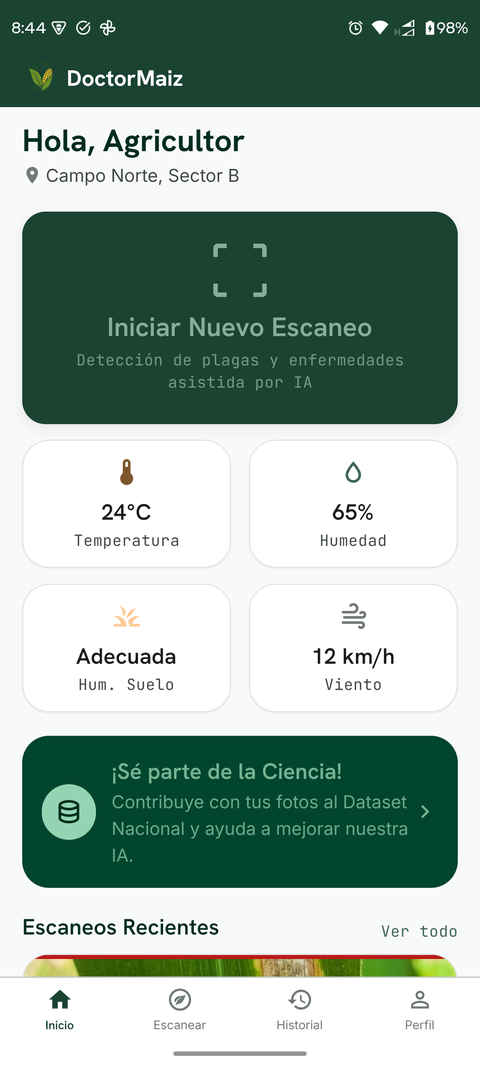
\includegraphics[width=0.148\textwidth]{app/home.png} &
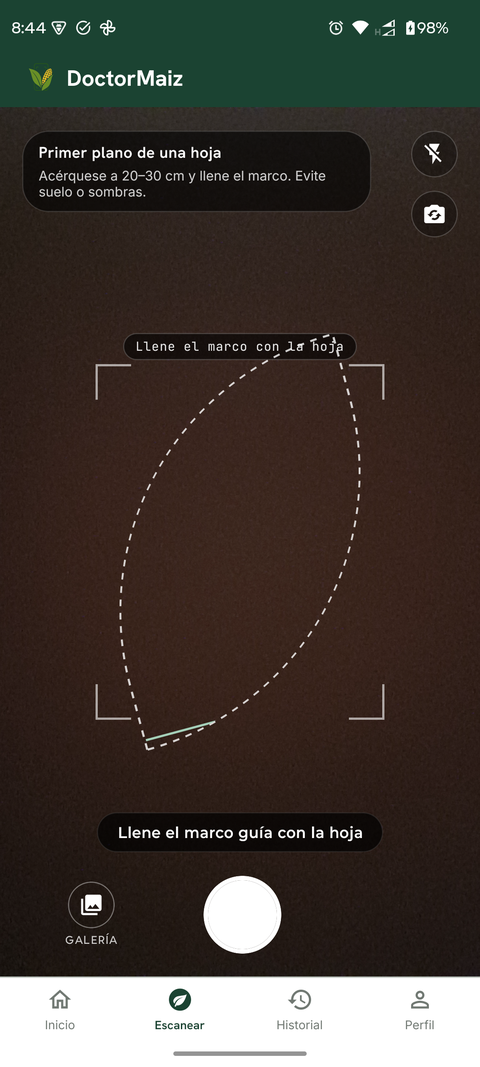
\includegraphics[width=0.148\textwidth]{app/camara-marco-guia.png} &
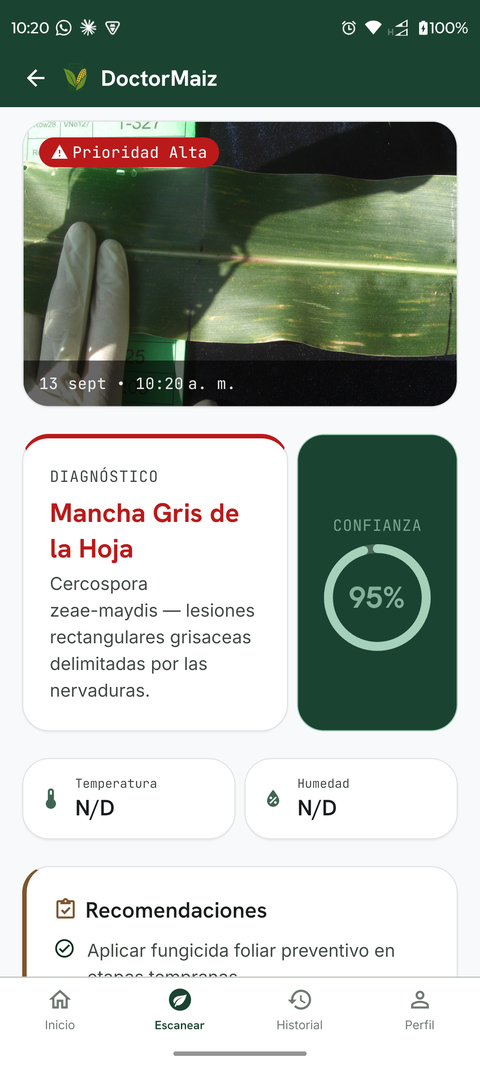
\includegraphics[width=0.148\textwidth]{app/resultado-mancha-gris.png} &
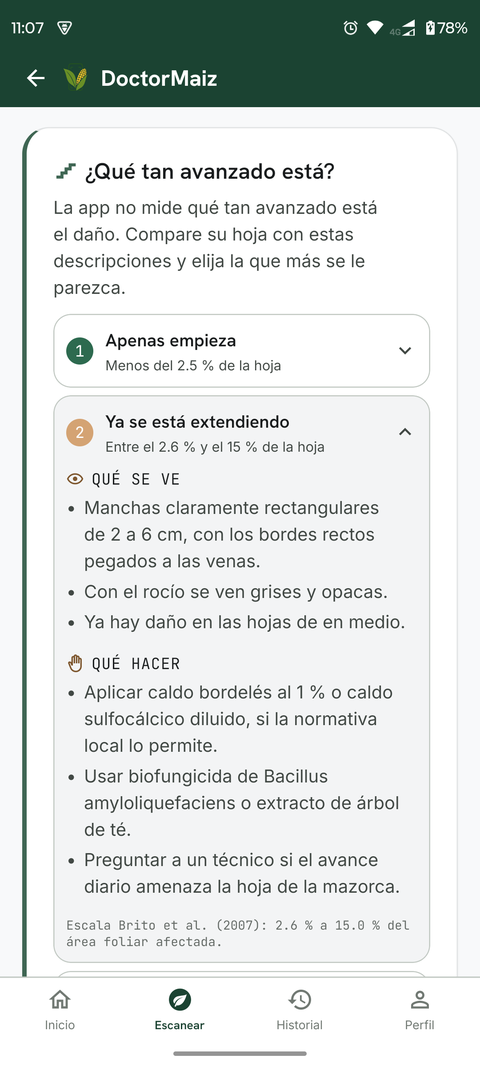
\includegraphics[width=0.148\textwidth]{app/resultado-severidad.png} &
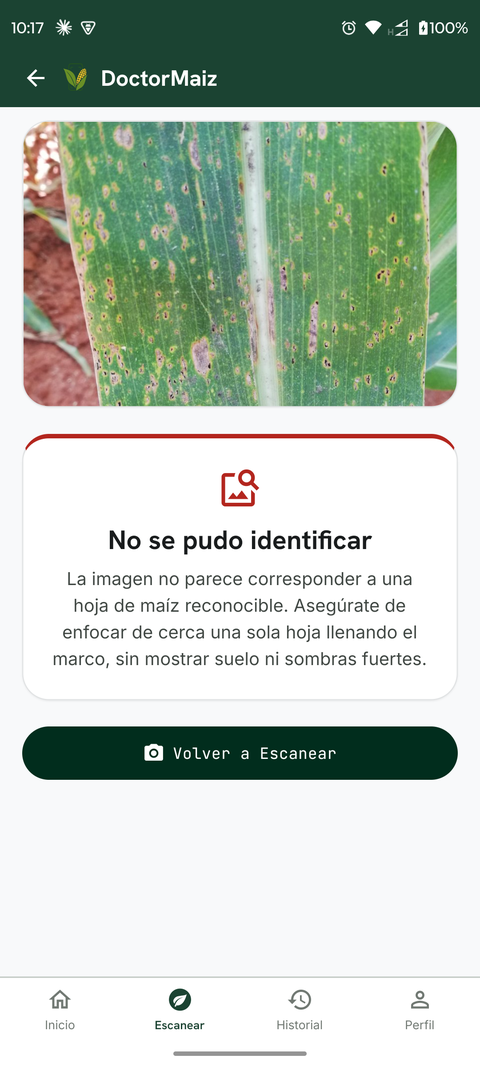
\includegraphics[width=0.148\textwidth]{app/resultado-no-reconocida.png} &
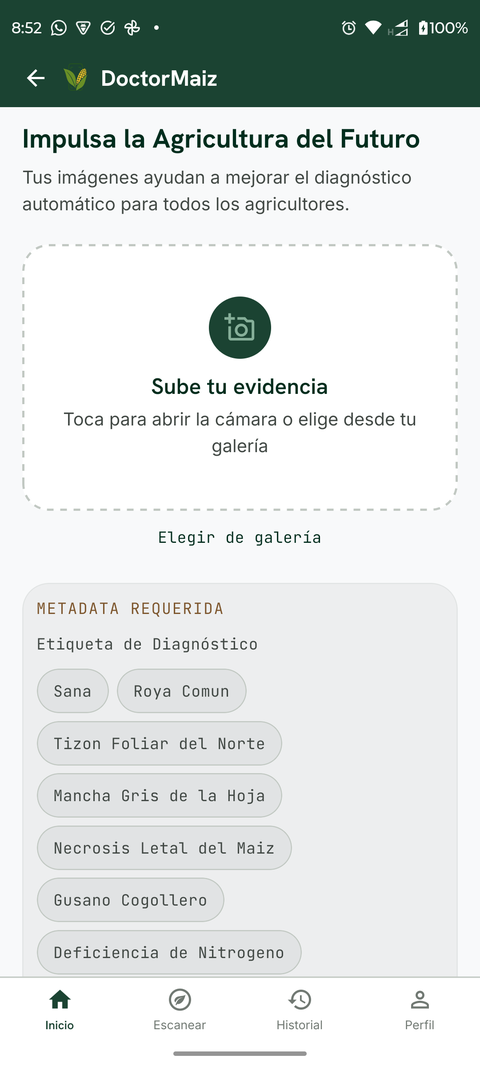
\includegraphics[width=0.148\textwidth]{app/contribuir.png} \\
\footnotesize (a) Inicio & \footnotesize (b) Marco guía & \footnotesize (c) Diagnóstico & \footnotesize (d) Guía de severidad & \footnotesize (e) Imagen no reconocida & \footnotesize (f) Aportes
\end{tabular}
\caption{Pantallas de la aplicación DoctorMaíz.}
\label{fig:app}
\end{figure*}

\section{Discusión}\label{sec:discusion}

\subsection{Dentro y fuera de la partición}
Los resultados admiten dos lecturas que no se contradicen. Dentro de la partición estratificada, el modelo cumple los criterios de diseño, la cuantización no le resta desempeño y la respuesta en el teléfono queda muy por debajo de la meta de 300\,ms. Fuera de ella, tres evidencias independientes apuntan en la misma dirección. El Macro \Fone{} cae a 0.6026 con fuentes no vistas, el modelo acierta 41 de 97 fotografías de campo externas y conserva la mayor parte de su exactitud viendo solo el borde de la imagen. Parte de lo aprendido es propio de los repositorios de origen, como el fondo, la iluminación o la cámara, y no de la enfermedad, lo que coincide con lo observado en otros conjuntos agrícolas \cite{ahmad2023,noyan2022}.

Esto explica por qué ni la búsqueda de hiperparámetros ni el ensamble cambiaron el panorama. Ambos optimizan sobre la misma distribución mezclada, y la mejora del ensamble (menos de un punto de Macro \Fone{}) no justifica ejecutar tres redes en el teléfono. La asociación entre fuente y clase de la Tabla~\ref{tab:fuente_clase} es un problema de datos y no de capacidad del modelo. El recorte al marco guía reduce el fondo visible en la captura, pero no corrige lo que el modelo aprendió del fondo durante el entrenamiento.

\subsection{Lecciones del despliegue}\label{sec:lecciones}
Dos defectos del despliegue pasaron inadvertidos en la evaluación del servidor y solo aparecieron en el teléfono. El primero afectó a la cuantización. Con escalas por canal en la capa totalmente conectada final, el núcleo de TensorFlow Lite que usa el teléfono aplica una sola escala por tensor, de modo que los logits salían multiplicados por un factor distinto en cada clase, la confianza se saturaba en 100\% y la regla~\eqref{eq:abstencion} quedaba inactiva. El intérprete del servidor usaba un delegado que sí admite escalas por canal y ocultaba el error. La solución fue cuantizar esa capa por tensor y añadir una comprobación estructural del modelo exportado.

El segundo afectó al preprocesado. La aplicación reducía la fotografía a $224\times224$ en un solo paso bilineal sin prefiltrado, lo que producía \textit{aliasing} en fotografías de alta resolución, llegaba a cambiar la clase predicha y multiplicaba la puntuación del detector hasta hacerle rechazar hojas legítimas. Se sustituyó por una reducción por etapas seguida de un filtro bilineal con antialias que reproduce byte a byte el del entrenamiento. Con ello se alcanzó la paridad de 143 de 143 imágenes, a costa de elevar la mediana del preprocesado a 98\,ms. Ambos casos muestran que la paridad entre el modelo evaluado y el que ejecuta el teléfono debe verificarse en el dispositivo y no darse por supuesta.

\subsection{Amenazas a la validez}
\textit{Validez externa.} El corpus no contiene fotografías salvadoreñas y la aplicación no se probó con productores. El conjunto de campo externo es pequeño (unas diez fotografías por clase), por lo que sus cifras por clase son orientativas.

\textit{Validez de constructo.} El DIR solo puede calcularse sobre tres clases, y para la roya común descansa en 16 imágenes de campo. En la ablación, las dos regiones ocultas no tienen la misma superficie. La guía de severidad no mide el área afectada y su utilidad depende del criterio del productor.

\textit{Validez interna.} La partición oficial se generó con una sola semilla, y la evaluación LOSO cubrió dos fuentes. Las latencias se midieron en un único teléfono de gama media.

\subsection{Implicaciones para la adopción}
En su estado actual, DoctorMaíz es una herramienta de orientación y no de diagnóstico definitivo en la parcela. Antes de una adopción institucional conviene validar la aplicación con promotores del CENTA y fotografías de cada zona productora, crear con el Ministerio de Agricultura y Ganadería y la Universidad de El Salvador un banco nacional de imágenes, evaluar el uso de los aportes en un sistema de vigilancia fitosanitaria con reglas claras sobre los datos y la ubicación, capacitar a cooperativas y asociaciones comunales en el uso del marco guía y mantener el software bajo licencias abiertas.

\section{Conclusiones}\label{sec:conclusiones}
Se presentó DoctorMaíz, una aplicación que clasifica sin conexión nueve condiciones de la hoja de maíz en un teléfono de gama media, se abstiene ante imágenes que no reconoce y acompaña cada resultado con una guía de manejo. El modelo EfficientNet-Lite0 cuantizado a Int8 pesa 3.74\,MB, alcanza un Macro \Fone{} de 0.9489 en la partición de prueba y responde en 23\,ms de inferencia y 98\,ms de preprocesado.

El resultado más relevante es la diferencia entre ese desempeño y el que se obtiene con fuentes no vistas. La validación agrupada por fuente, la retención de fuentes completas, las fotografías de campo externas y la ablación espacial coinciden en que una partición estratificada sobrestima el desempeño en campo cuando la procedencia y la clase están asociadas. Es poco probable que otra arquitectura o más ajuste de hiperparámetros cierren esa brecha. Lo que falta son fotografías tomadas en parcelas salvadoreñas, y el módulo de aportes de la aplicación es el medio previsto para reunirlas. El trabajo futuro incluye reentrenar con esas imágenes evaluando siempre con fuentes completas fuera del entrenamiento, probar la aplicación con productores y técnicos, y reducir el tiempo de preprocesado en el teléfono.

\section*{Disponibilidad de datos y código}
El código de la cadena de entrenamiento, de la aplicación y de la API está disponible en \url{https://github.com/daiv05/maize-doctor-classifier}, \url{https://github.com/Edenilson-Molina/maize-doctor-app} y \url{https://github.com/daiv05/maize-doctor-api}. El corpus consolidado se publica en \url{https://huggingface.co/datasets/daiv05/corn-leaf-diseases-pests-and-deficiencies}, y cada fuente conserva su licencia original. La huella SHA-256 del modelo Int8 evaluado es \path{bb31467a58c11cd474159bd5739a7a57b1f1edfda6b5dbfae8fa91337f3c56b1}.

\section*{Agradecimientos}
Los autores agradecen a los docentes asesores Ing.~Bladimir Díaz Campos, Ing.~Karen Elvira Peñate Avilés e Ing.~Rodrigo Ernesto Vásquez Escalante, y a la Escuela de Ingeniería de Sistemas Informáticos de la Universidad de El Salvador.

\bibliographystyle{IEEEtran}
\bibliography{referencias}

\end{document}
